\chapter{Modelo de datos a implementar en tareas posteriores}

A continuación se muestran los modelos de datos que los autores han creado para dar soporte a las tareas posteriores luego de terminar el prototipo en el presente proyecto.


\section{Modelo de datos de gestión de estadísticas}

En \cite{dependent_time_graphs}, se da una explicación acerca de un patrón llevado a cabo para la recolección de datos basados en tiempo (timestamp). Para la gestión de estadísticas se hace necesario llevar acabo éste patrón debido a que se debe guardar las interacciones de los usuarios con ubicaciones deportivas (cuando los usuarios van a practicar deporte en determinada ubicación). Debido a eso, se implementó un frame temporal llamado E\_FrameDia que guarda la hora de llegada y de salida de una ubicación deportiva por parte de un usuario. Asimismo, fue creada la entidad E\_RunDia para accesar al día de la semana que se quisiera, el cual estará a todos los timestamp que se vayan generando a través del tiempo. En la figura \ref{fig:modelo_datos_gestion_estadisticas} es posible ver las entidades E\_FrameDia con las horas y la entidad E\_RunDia con un id generado por Neo4j. En éste caso, dicho E\_RunDia actúa como el día lunes. También se pueden observar los nodos Usuario y UbicaciónUsuario conectandose a través de dicho frame de tiempo.

\begin{figure}[!htb]
  \begin{center}
    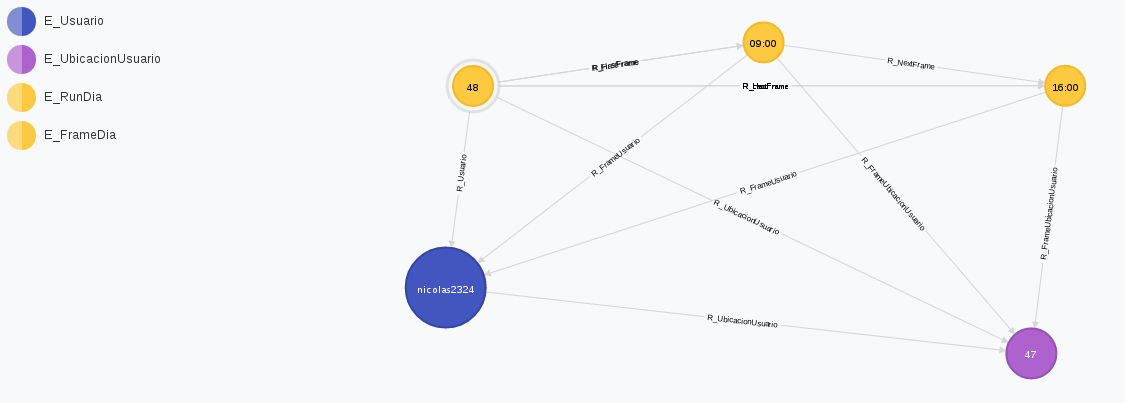
\includegraphics[width=11cm]{./imagenes/Modelo_de_datos/Gestion_estadisticas.png}
    \caption{Modelo de datos de gestión de estadisticas}
    \label{fig:modelo_datos_gestion_estadisticas}
    \textbf{Fuente:}  Autores \\
    \textbf{Ver anexo en:} /Proyecto/imagenes/Modelo\_de\_datos/Gestion\_estadisticas.png
  \end{center}
\end{figure}

Los nodos que hacen referencia a relaciones n-arias son mostrados en gris.

\section{Modelo de datos de gestión de conocimiento}

En esta parte del modelo se puede observar como se representa la base de conocimientos de la aplicación. Esta base de conocimientos es almentada por los mismos usuarios que son quienes estan encargados de crear y discutir los diferentes contenidos que existan. Los contenidos pueden ser explicados con elementos multimedia que el usuario creador está encargado de proporcionar.

\begin{figure}[!htb]
  \begin{center}
    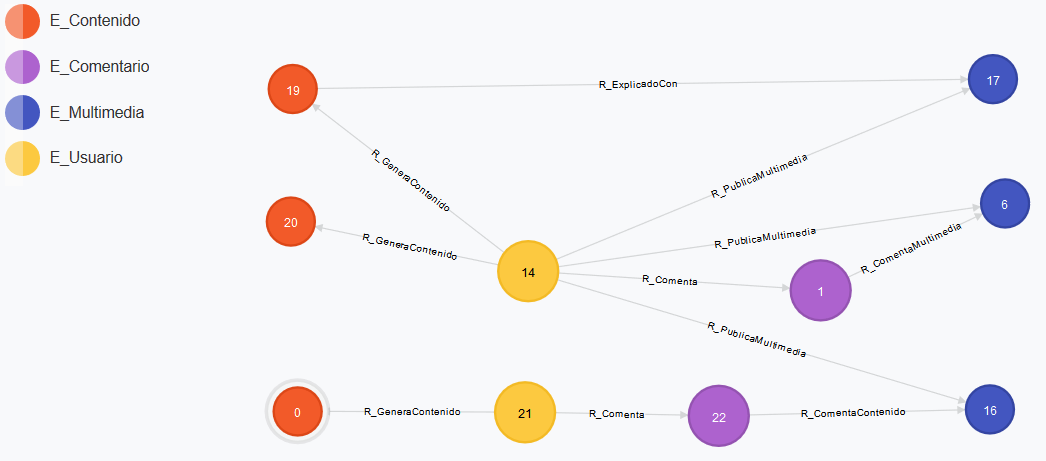
\includegraphics[width=11cm]{./imagenes/Modelo_de_datos/Contenidos.png}
    \caption{Modelo de datos de gestión del conocimiento}
    \label{fig:modelo_datos_gestion_conocimiento}
    \textbf{Fuente:}  Autores \\
    \textbf{Ver anexo en:} /Proyecto/imagenes/Modelo\_de\_datos/Contenidos.png
  \end{center}
\end{figure}

\section{Modelo de datos de gestión de multimedia}

Para esta seccion cabe destacar la funcion de los nodos E\_Multimedia. Estos nodos representan un contenido multimedia que puede ser utilizado en los diferentes módulos de la aplicaicón. Toda interacción con los elementos multimedia E\_Foto y E\_Video se debe hacer a través de los nodo E\_Multimedia (Comentar, referenciar, compartir). Adicionalmente, los elementos E\_Album agrupan una serie de Fotos de un usuario.

\begin{figure}[!htb]
  \begin{center}
    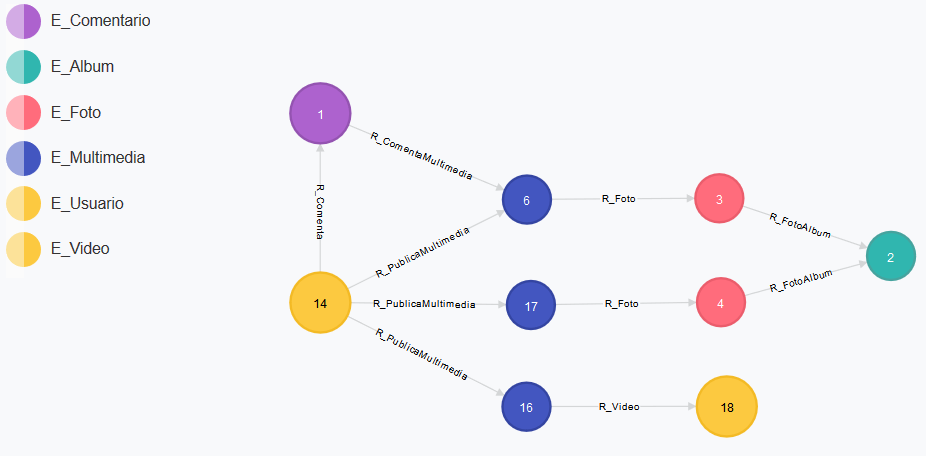
\includegraphics[width=11cm]{./imagenes/Modelo_de_datos/Multimedia.png}
    \caption{Modelo de datos de gestión de multimedia}
    \label{fig:modelo_datos_gestion_multimedia}
    \textbf{Fuente:}  Autores \\
    \textbf{Ver anexo en:} /Proyecto/imagenes/Modelo\_de\_datos/Multimedia.png
  \end{center}
\end{figure}

\section{Modelo de datos de gestión de roles}

En esta sección del modelo se parametrizan los diferentes roles existentes en la aplicación. Cada rol tiene asociados una serie de permisos que le brindan diferentes funcinalidades al usuario que asuma el rol respectivo.

\begin{figure}[!htb]
  \begin{center}
    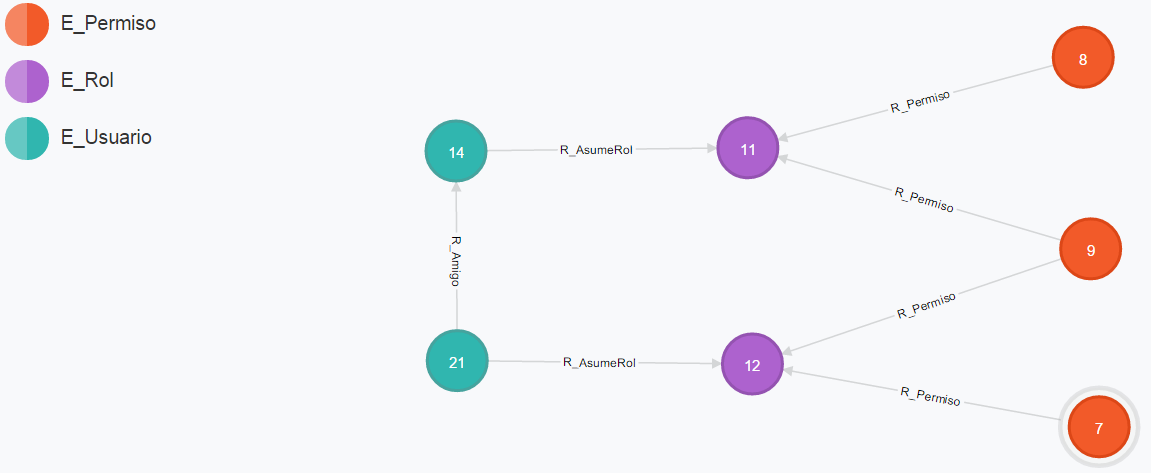
\includegraphics[width=11cm]{./imagenes/Modelo_de_datos/Roles.png}
    \caption{Modelo de datos de gestión de roles}
    \label{fig:modelo_datos_gestion_roles}
    \textbf{Fuente:}  Autores \\
    \textbf{Ver anexo en:} /Proyecto/imagenes/Modelo\_de\_datos/Roles.png
  \end{center}
\end{figure}